\section{RESEARCH METHODOLOGY}
\hspace{1.27cm}
The experiment of path planning and control for the mobile robot consists of many steps. First, the mobile robot model and sensor model are built to use inside the simulation software. Second, using the ROS packages Hector SLAM and Gmapping SLAM, the occupancy grid map is built. Third, after the occupancy grid map is built, the A* path planning algorithm is applied to get the trajectory from the start point to the goal point. Finally, the robot movement is controlled to the reference trajectory using backstepping controller algorithm and tuning parameters for smooth motion. \textbf{\figureautorefname{ \ref{fig:Workflow}}} presents the overall workflow of the project.\par

% Figure Image =============================================================================
\begin{figure}[ht]
	\centering
	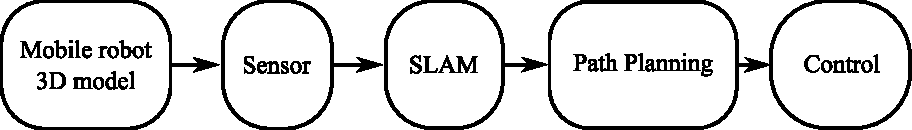
\includegraphics[scale=1]{images/imagess/3method-workflow.pdf}
	\caption{Workflow}
	\label{fig:Workflow}
\end{figure}
% Figure Image =============================================================================

\subsection{Mobile Robot 3D Modelling}
\hspace{1.27cm}
The robot model in constructed in Gazebo simulation. Gazebo uses the robot model written in SDF format. We construct the robot model with the parameters below: \par

$\bullet$ \textbf{Robot Base} (\textbf{\figureautorefname{ \ref{fig:Mobile Robot Base}}})\par
The model base dimensions are:
\begin{itemize}
	\item {\makebox[2cm]{Length\hfill} = 0.4 $m$}
	\item {\makebox[2cm]{Width\hfill} = 0.2 $m$}
	\item {\makebox[2cm]{Height\hfill} = 0.1 $m$}
%    \item Length = 0.4$m$
%    \item Width = 0.2$m$
%    \item Height = 0.1$m$
\end{itemize}

% Figure Image =============================================================================
\begin{figure}[ht]
	\centering
	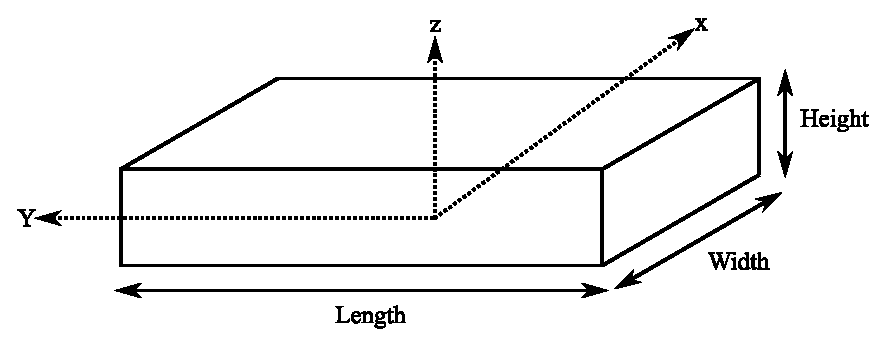
\includegraphics[scale=1]{images/imagess/3method-imu.eps}
	\caption{Mobile Robot Base}
	\label{fig:Mobile Robot Base}
\end{figure}
% Figure Image =============================================================================
\break
$\bullet$ \textbf{Wheels and Caster Wheels} (\textbf{\figureautorefname{ \ref{fig:Mobile Robot Wheel and Caster Wheel}}})\par
The robot wheels and caster wheel dimensions are:
\begin{itemize}
	\item {\makebox[4cm]{Wheel radius\hfill} = 0.1 $m$}
	\item {\makebox[4cm]{Wheel width\hfill} = 0.05 $m$}
	\item {\makebox[4cm]{Caster wheel radius\hfill} = 0.05 $m$}
%    \item Wheel radius = 0.1m
%    \item Wheel width = 0.015m
%    \item Caster wheel radius = 0.25m
\end{itemize}

% Figure Image =============================================================================
\begin{figure}[ht]
	\centering
	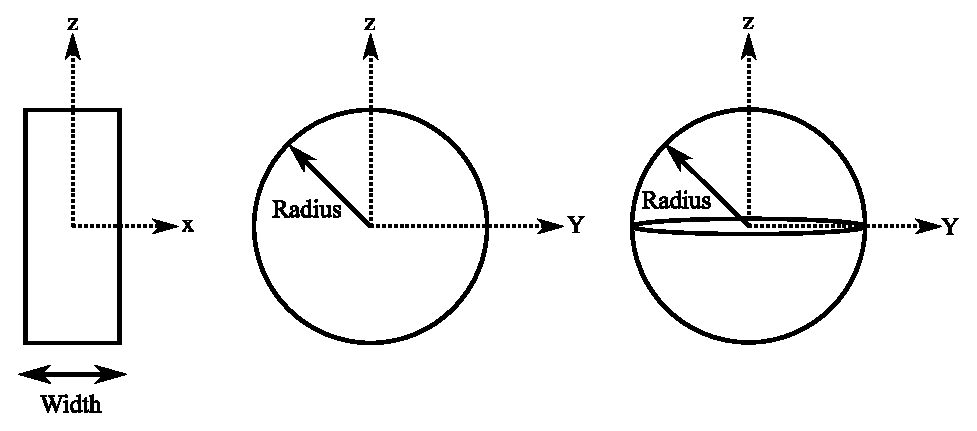
\includegraphics[scale=0.9]{images/imagess/3method-wheel.eps} 
	\caption{Mobile Robot Wheel and Caster Wheel}
	\label{fig:Mobile Robot Wheel and Caster Wheel}
\end{figure}
% Figure Image =============================================================================

\subsection{Sensor 3D Modelling}
\hspace{1.27cm}
The robot is equipped with Lidar sensor, with the max range of 10 $m$, min range of 0.1 $m$, 360$^{\circ}$ field of view, and resolution of 0.1$^{\circ}$. The IMU is attached to the robot frame with the z-axis pointing upward. The sensor noise is included in the simulation with the model of zero-mean Gaussian white. \textbf{\figureautorefname{ \ref{fig:Mobile Robot Modelling Side and Top View}}} illustrates the mobile robot model side and top view.\par

$\bullet$ \textbf{Lidar} (\textbf{\figureautorefname{ \ref{fig:Lidar Dimension}}})\par
The Lidar dimensions are:
\begin{itemize}
	\item {\makebox[3cm]{Diameter\hfill} = 0.065 $m$}
	\item {\makebox[3cm]{Height\hfill} = 0.070 $m$}
	\item {\makebox[3cm]{Height to Laser\hfill} = 0.055 $m$}
%    \item Diameter = 0.1m
%    \item Height = 0.015m
%    \item Height to Laser = 0.25m
\end{itemize}

$\bullet$ \textbf{IMU} (\textbf{\figureautorefname{ \ref{fig:IMU Dimension}}})\par
The IMU dimensions are:
\begin{itemize}
	\item {\makebox[2cm]{Length\hfill} = 0.02 $m$}
	\item {\makebox[2cm]{Width\hfill} = 0.01 $m$}
	\item {\makebox[2cm]{Height\hfill} = 0.01 $m$}
%    \item Length = 0.4m
%    \item Width = 0.2m
%    \item Height = 0.1m
\end{itemize}

% Figure Image =============================================================================
\begin{figure}[ht]
	\centering
	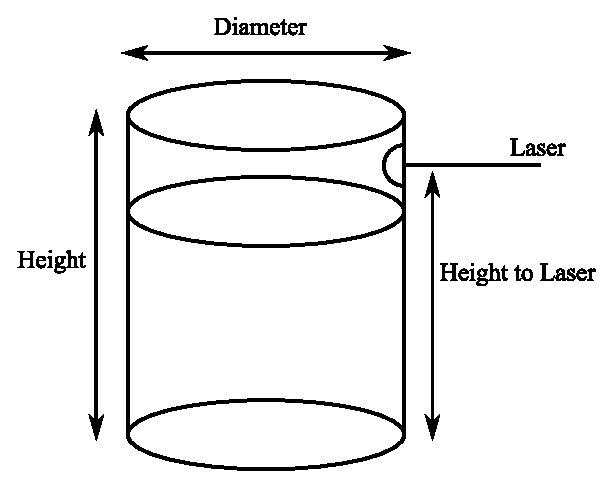
\includegraphics[scale=1]{images/imagess/3method-lidar.eps} 
	\caption{Lidar Dimension}
	\label{fig:Lidar Dimension}
\end{figure}
% Figure Image =============================================================================

% Figure Image =============================================================================
\begin{figure}[ht]
	\centering
	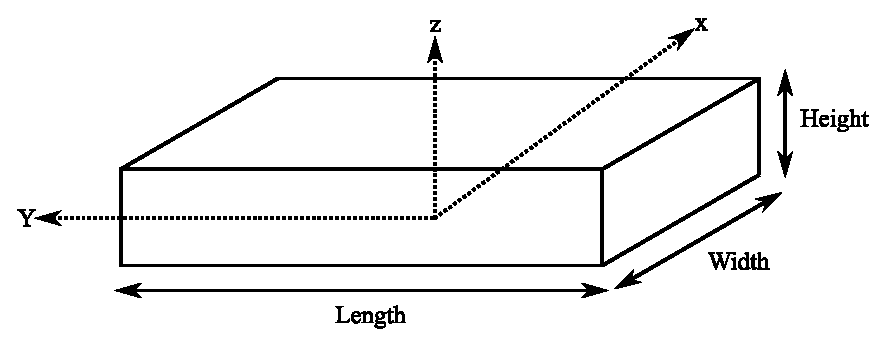
\includegraphics[scale=1]{images/imagess/3method-imu.eps} 
	\caption{IMU Dimension}
	\label{fig:IMU Dimension}
\end{figure}
% Figure Image =============================================================================

% Figure Image =============================================================================
\begin{figure}[H]
	\centering
	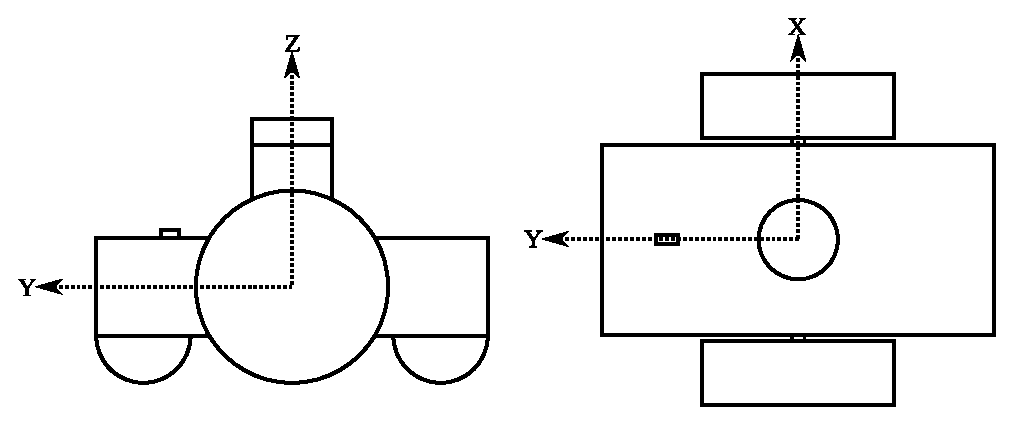
\includegraphics[scale=1]{images/imagess/3method-top-side-view.eps} 
	\caption{Mobile Robot Modelling Side and Top View}
	\label{fig:Mobile Robot Modelling Side and Top View}
\end{figure}
% Figure Image =============================================================================





\subsection{SLAM}
% Figure Image =============================================================================
\begin{figure}[ht]
	\centering
	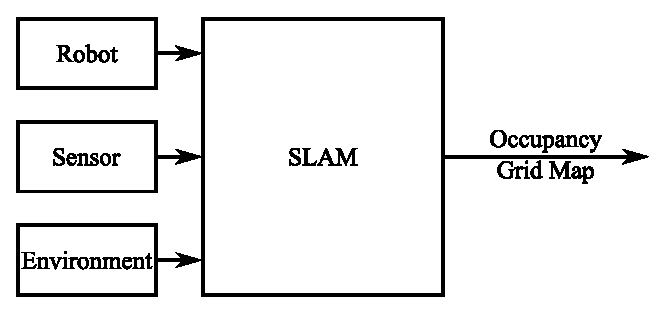
\includegraphics[scale=1]{images/imagess/3method-slam.eps} 
	\caption{SLAM}
	\label{fig:SLAM}
\end{figure}
% Figure Image =============================================================================
\hspace{1.27cm}
\textbf{\figureautorefname{ \ref{fig:SLAM}}}, the SLAM method is used to create the Occupancy Grid Map. In Gazebo, first we create a simulation of the indoor environment. Second, we load the robot model and sensor from the SDF file that is created in the Gazebo. Using ROS plug-in for Gazebo, the robot is controlled with the keyboard input. The robot is driven around while the SLAM is running to create the Occupancy Grid Map of the environment.\par



\subsection{Path Planning and Control}
% Figure Image =============================================================================
\begin{figure}[ht]
	\centering
	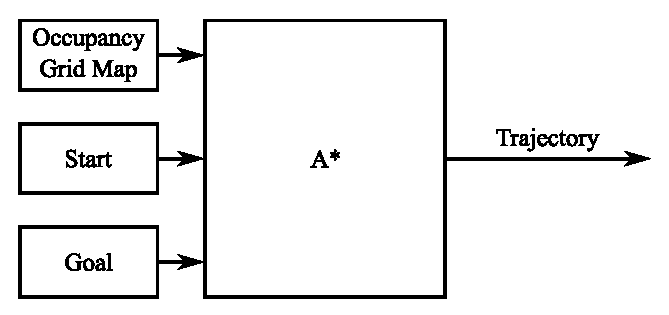
\includegraphics[scale=1]{images/imagess/3method-astar.eps} 
	\caption{Path Planning of Astar}
	\label{fig:Path Planning of Astar}
\end{figure}
% Figure Image =============================================================================
\hspace{1.27cm}
\textbf{\figureautorefname{ \ref{fig:Path Planning of Astar}}}, given the Occupancy Grid Map, the path planning algorithm is used for the calculation of  the reference trajectory for the robot to move. The reference trajectory then is given to the robot which is controlled by the backstepping trajectory tracking algorithm. The control input from the backstepping is publishing on to the ROS control topic to determine the torque of each wheel of the robot to move. In every time-step, the robot pose is estimate using the extended kalman filter sensor fusion algorithm. The pose of the robot is plotted against the reference pose.\par


\hspace{1.27cm}
\textbf{\figureautorefname{ \ref{fig:Map1}}} and \textbf{\figureautorefname{ \ref{fig:Map2}}} are the model of simulated rooms for experiment and its dimension. In this research, we use 2 simulated room model and named it: "Map1" and "Map2". In these 2 figures, the yellow spot represents the Start location for the robot, the green spot represents the goal location where the robot will move to.\\
$\bullet$ \textbf{Indoor 3D models: "Map1"}\par
% Figure Image =============================================================================
\begin{figure}[H]
	\centering
	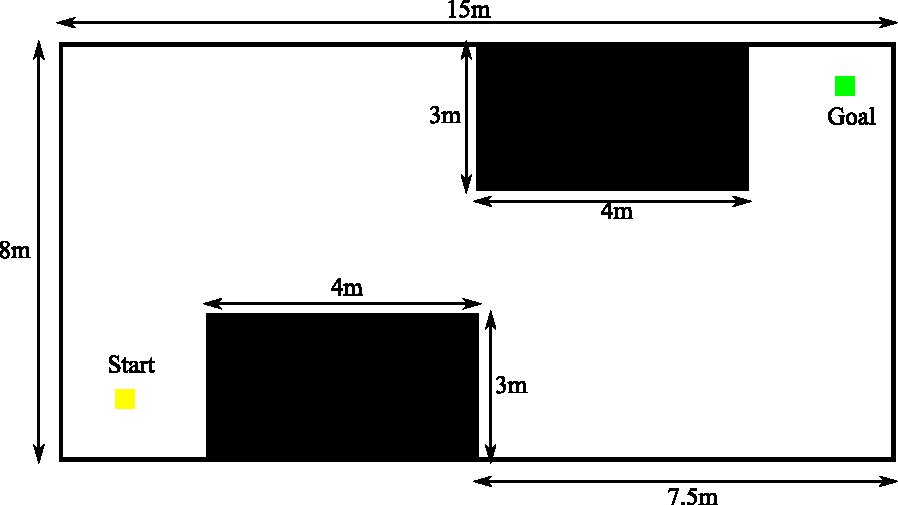
\includegraphics[scale=1]{images/imagess/3method-map1.pdf} 
	\caption{"Map1" Model}
	\label{fig:Map1}
\end{figure}
% Figure Image =============================================================================

$\bullet$ \textbf{Indoor 3D models: "Map2"}\par
% Figure Image =============================================================================
\begin{figure}[H]
	\centering
	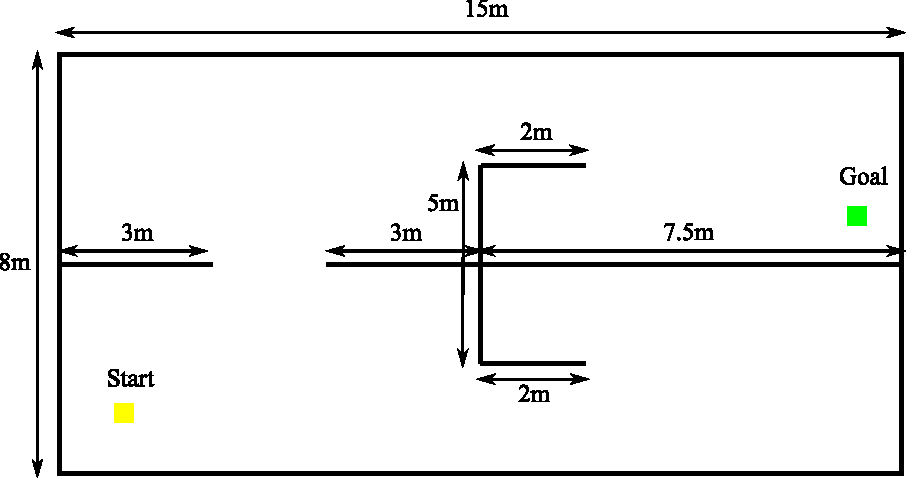
\includegraphics[scale=1]{images/imagess/3method-map2.pdf} 
	\caption{"Map2" Model}
	\label{fig:Map2}
\end{figure}
% Figure Image =============================================================================